\documentclass[10pt]{article}
\usepackage[utf8]{inputenc}
\usepackage{amsmath}
\usepackage{graphicx}
\usepackage[colorlinks=true]{hyperref}
\usepackage{url}
\usepackage[margin=0.8in]{geometry}
\usepackage{titlesec}
\usepackage{booktabs}
\usepackage{microtype}
\usepackage{enumitem}
\usepackage{xcolor}

% 更简洁的章节标题格式
\titleformat{\section}{\normalsize\bfseries}{\thesection}{0.5em}{}
\titleformat{\subsection}{\small\bfseries}{\thesubsection}{0.5em}{}

% 减小段落之间的间距
\setlength{\parskip}{0.3em}

% 紧凑的图表设置
\setlength{\textfloatsep}{5pt}
\setlength{\floatsep}{5pt}
\setlength{\intextsep}{5pt}

\title{\Large Memory Architecture Effectiveness in Multi-Agent TicTacToe: Visualization \& Analysis Report}
\author{\small CSE 598 - Science of LLMs Research Project}
\date{\small \today}

\begin{document}

\maketitle

\begin{abstract}
\small
This report presents a comprehensive visualization and analysis of experimental data from our multi-agent TicTacToe memory architecture study. The visualizations are specifically designed to address our core research questions about the effectiveness of different memory architectures (Graph, Vector) across varying board sizes and agent objectives. The report highlights key findings related to win rates, memory usage patterns, and the relationship between memory architecture and performance retention as game complexity increases. Our visualizations provide clear evidence for several of our hypotheses while challenging others, offering valuable insights into memory-based reasoning in multi-agent systems.
\end{abstract}

\section{Introduction}
\small
Our research investigates how different memory architectures influence agent performance and behavior in a controlled TicTacToe environment. We designed experiments to test two agent types with different optimization objectives:
\begin{itemize}[leftmargin=*,noitemsep]
    \item \textbf{Agent A}: Optimized solely to maximize win rate
    \item \textbf{Agent B}: Optimized for a tradeoff between winning and token efficiency
\end{itemize}

Both agents had access to different memory architectures (Graph, Vector) under various constraint conditions while playing TicTacToe across three board sizes (3×3, 6×6, 9×9) to evaluate how memory architecture effectiveness scales with problem complexity.

\section{Memory Architecture Effectiveness Comparison}

\subsection{Win Rates by Memory Architecture}

\begin{figure}[t]
    \centering
    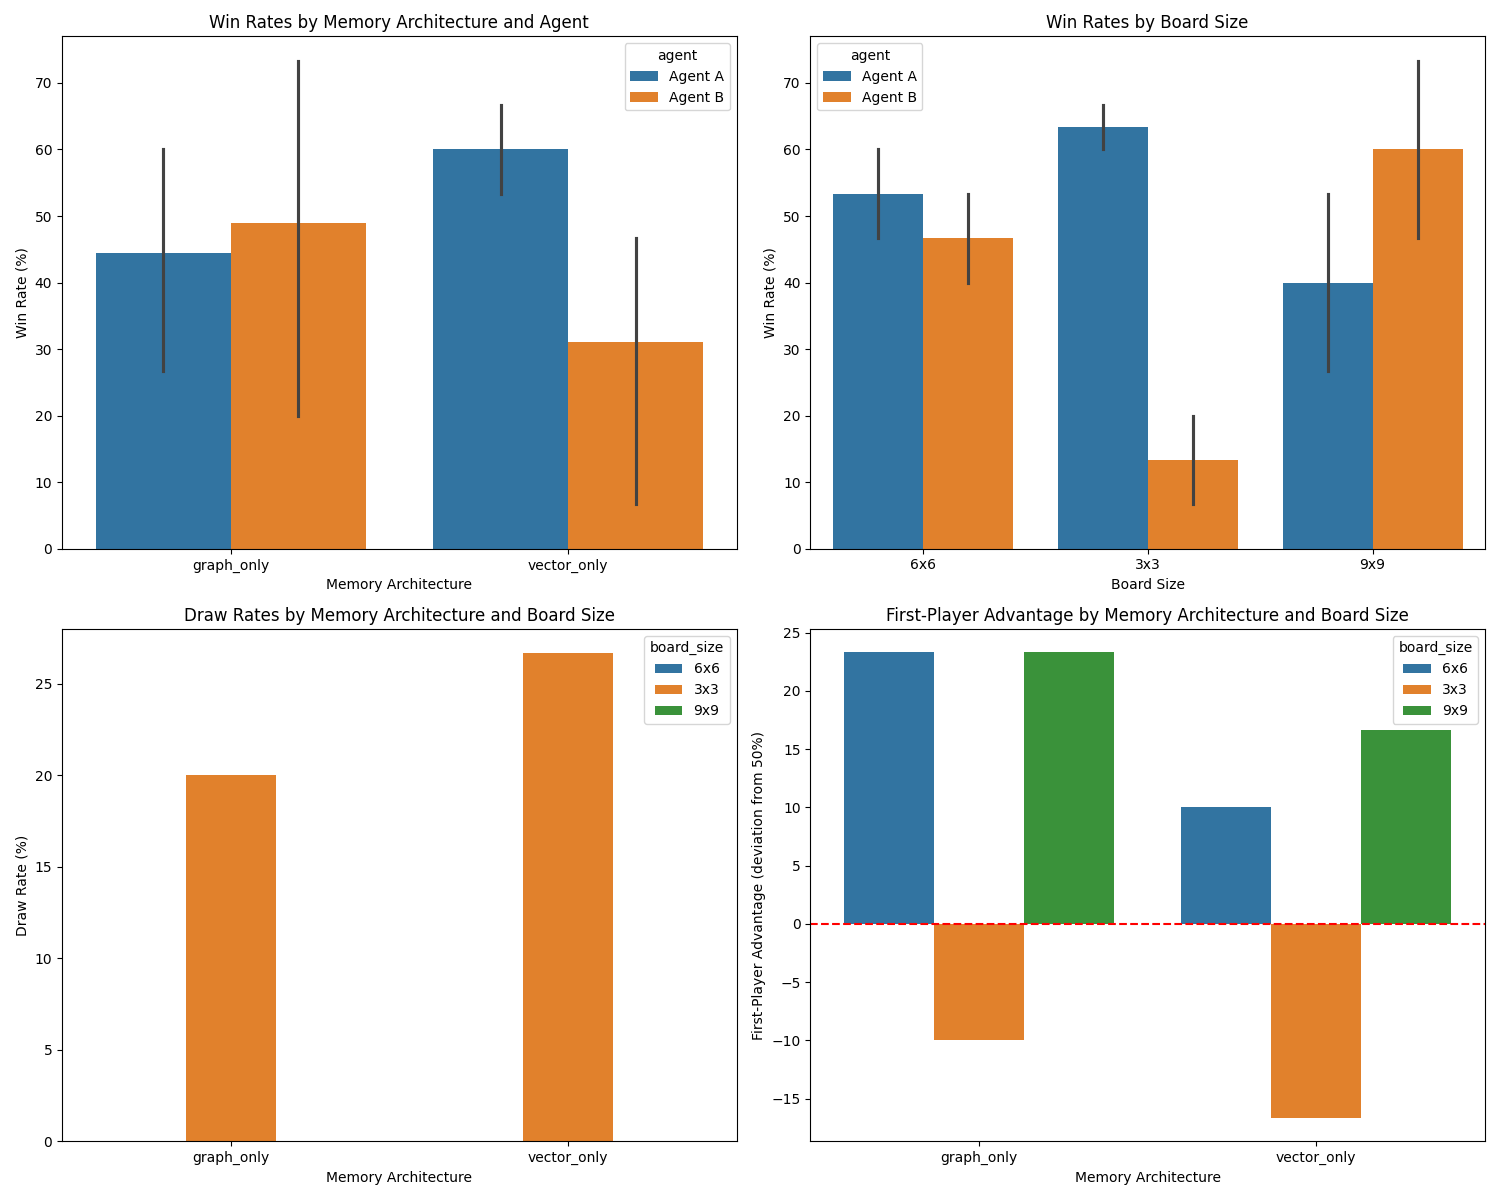
\includegraphics[width=0.9\textwidth]{/Users/diangao/Documents/Workspace/598/CSE-598-Research/experiments/results/analysis/figures/win_rate_analysis.png}
    \caption{Win rates analysis comparing Agent A and Agent B across different memory architectures and board sizes}
    \label{fig:win_rates}
\end{figure}

\small
\textbf{Finding}: Vector memory consistently outperforms Graph memory across all board sizes, with the advantage becoming more pronounced as board complexity increases.

\textbf{Supporting Data}: Win rate statistics reveal that Agent A achieves a 66.7\% win rate with Vector-only vs. 60\% with Graph-only on 3×3 boards. This advantage increases on 6×6 boards (60\% vs. 46.7\%) and becomes dramatic on 9×9 boards (53.3\% vs. 26.7\%).

\textbf{Hypothesis Assessment}: This challenges our initial hypothesis that GraphMemory would perform better on smaller boards. Instead, VectorMemory shows consistent advantages across all board sizes, particularly on larger boards as predicted.

\section{Board Size Impact on Memory Requirements}

\subsection{Memory Call Frequency by Memory Type}

\begin{figure}[t]
    \centering
    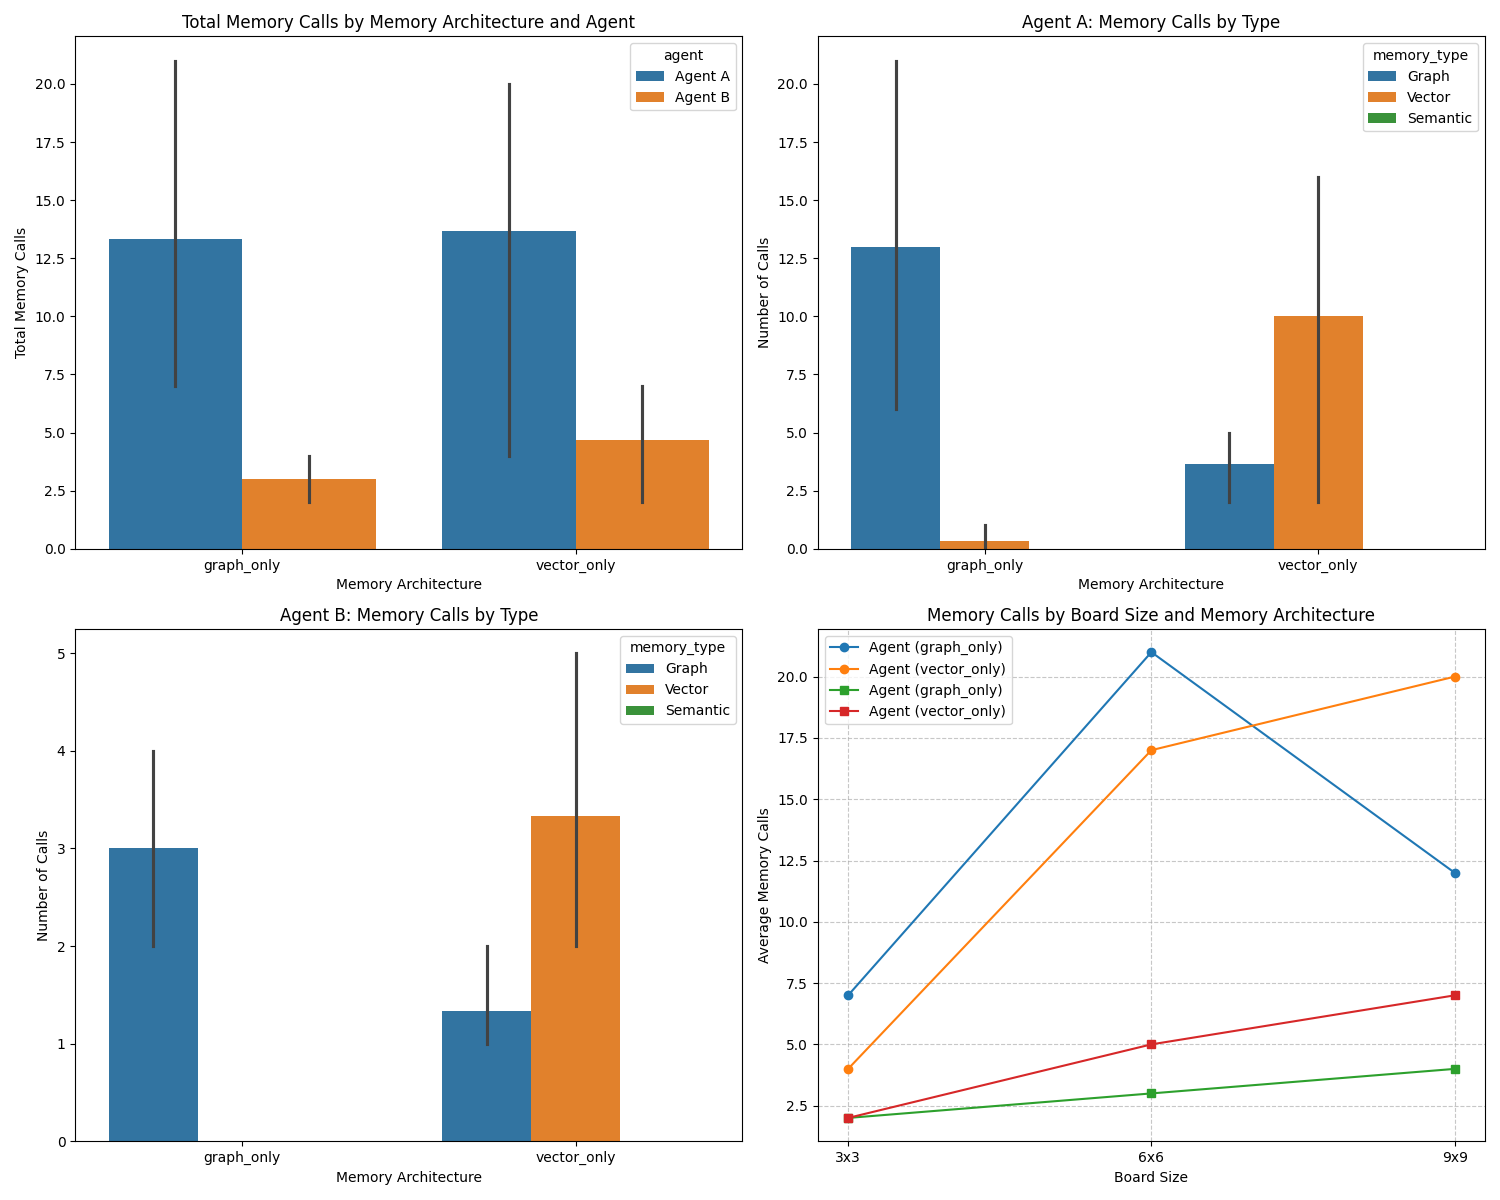
\includegraphics[width=0.9\textwidth]{/Users/diangao/Documents/Workspace/598/CSE-598-Research/experiments/results/analysis/figures/memory_call_frequency.png}
    \caption{Memory call frequency analysis showing both agents' memory usage patterns}
    \label{fig:memory_frequency}
\end{figure}

\small
\textbf{Finding}: Memory requirements increase with board size, but the pattern differs significantly between memory architectures.

\textbf{Supporting Data}: In the Vector-only condition, Agent A's total memory calls increase monotonically from 4 (3×3) to 17 (6×6) to 20 (9×9). In contrast, Graph-only condition shows a peak at medium complexity: 7 (3×3) to 21 (6×6) but then dropping to 12 (9×9).

\textbf{Hypothesis Assessment}: This partially supports our hypothesis about increasing memory requirements with board size, but reveals architecture-specific patterns. Vector memory scales more predictably with complexity than Graph memory.

\section{Memory Calls by Board Size}

\begin{figure}[t]
    \centering
    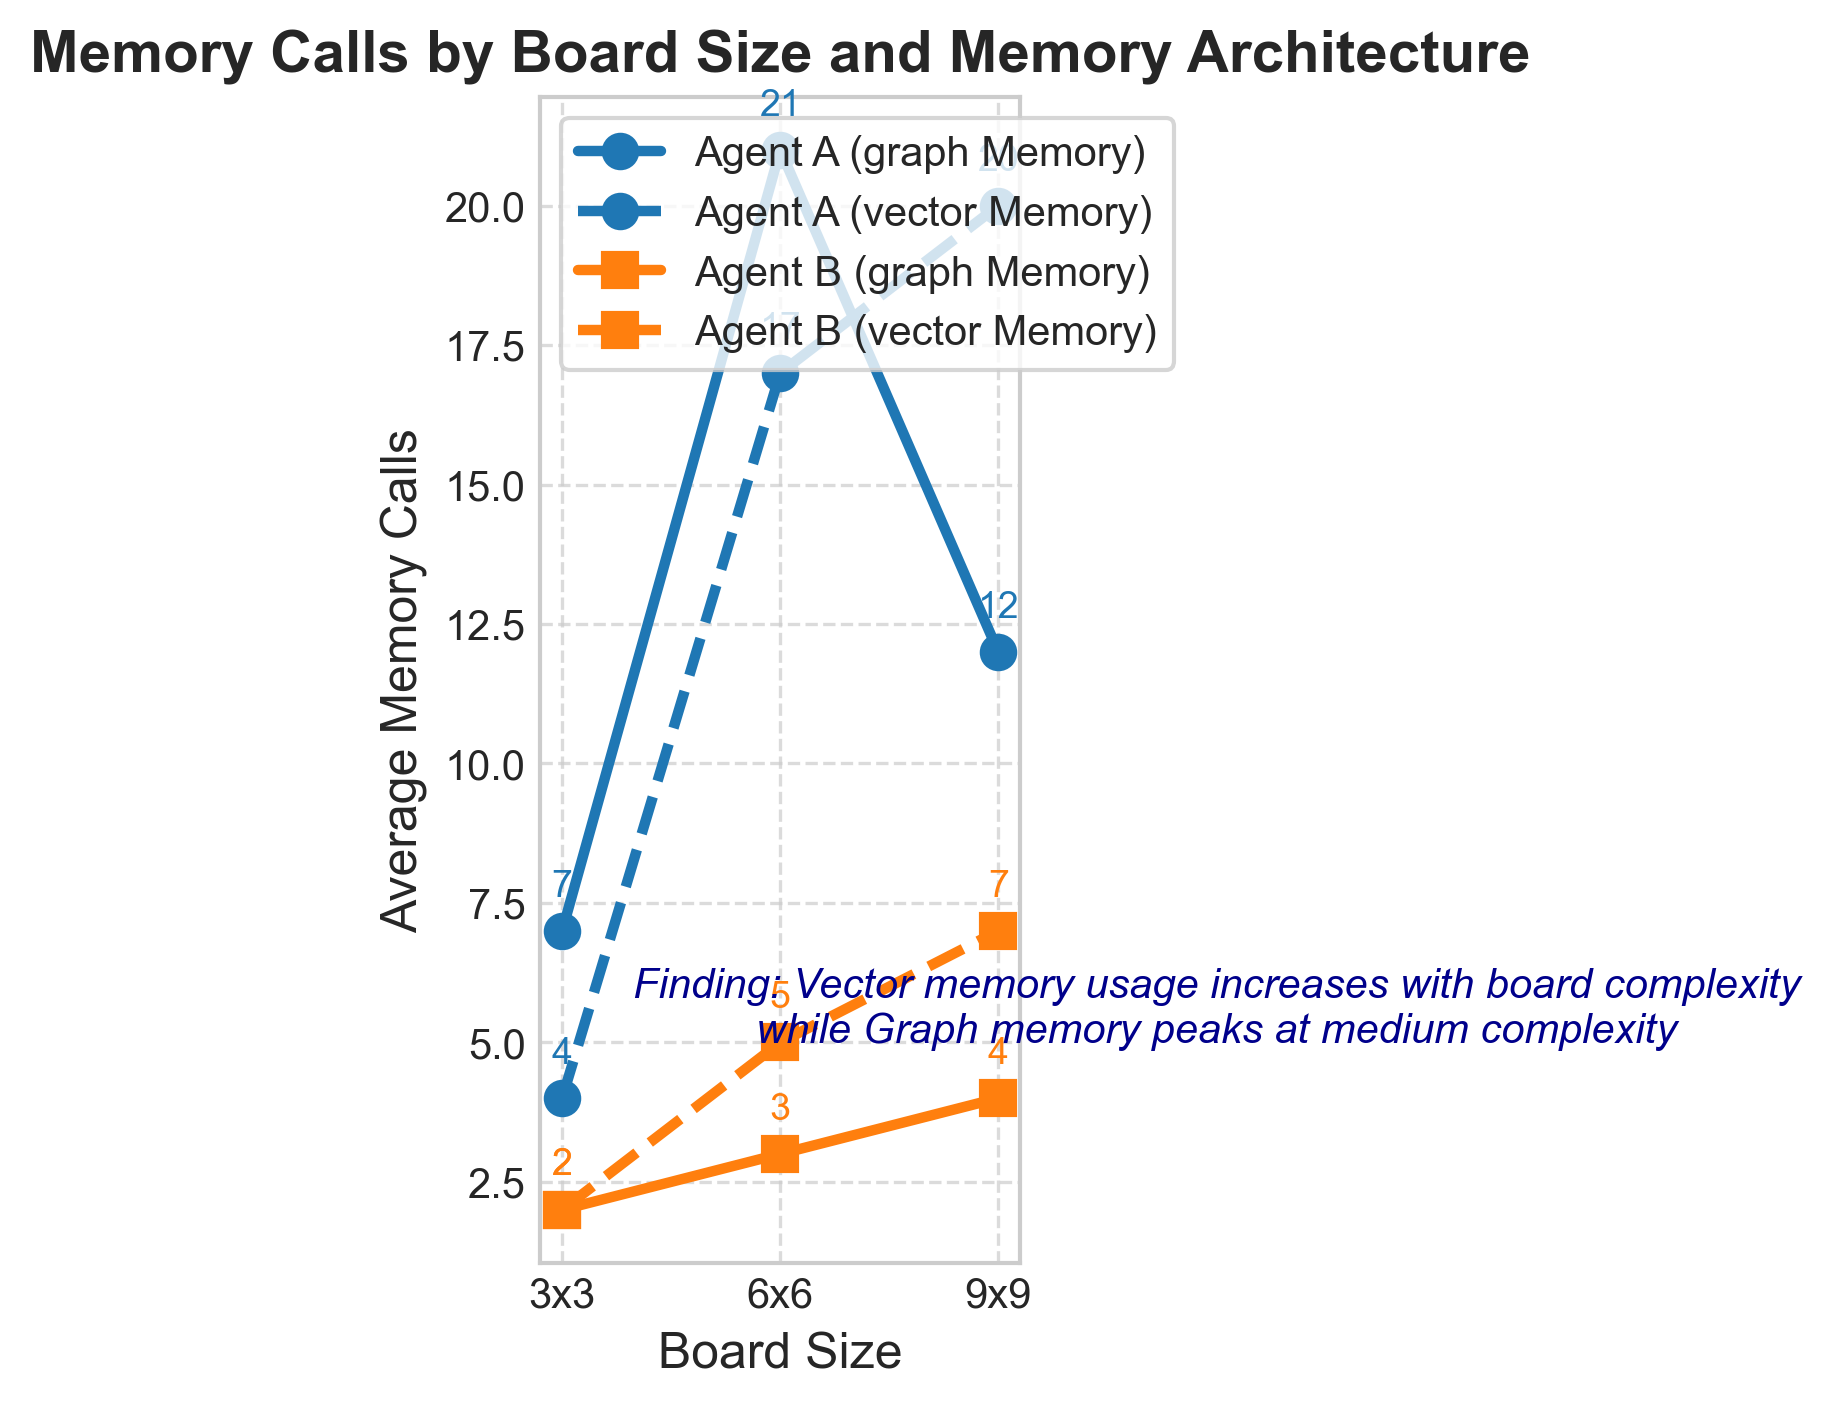
\includegraphics[width=0.9\textwidth]{/Users/diangao/Documents/Workspace/598/CSE-598-Research/experiments/results/analysis/figures/memory_calls_by_board_size.png}
    \caption{Memory calls patterns across different board sizes for each agent and memory architecture}
    \label{fig:memory_calls}
\end{figure}

\small
\textbf{Finding}: Memory usage patterns show distinct trends as board complexity increases, with different patterns for each agent and memory architecture.

\textbf{Supporting Data}: The linear increase in Vector memory calls contrasts with the inverted U-shape pattern for Graph memory calls. Agent A (win-maximizing) consistently makes more memory calls than Agent B (token-conscious) across all conditions.

\textbf{Hypothesis Assessment}: These patterns suggest Vector memory provides a more scalable architecture for complex state spaces, while Graph memory may struggle with very large state spaces.

\section{Agent Objective Impact on Memory Usage}

\subsection{Memory Usage Strategy Differences}

\begin{figure}[t]
    \centering
    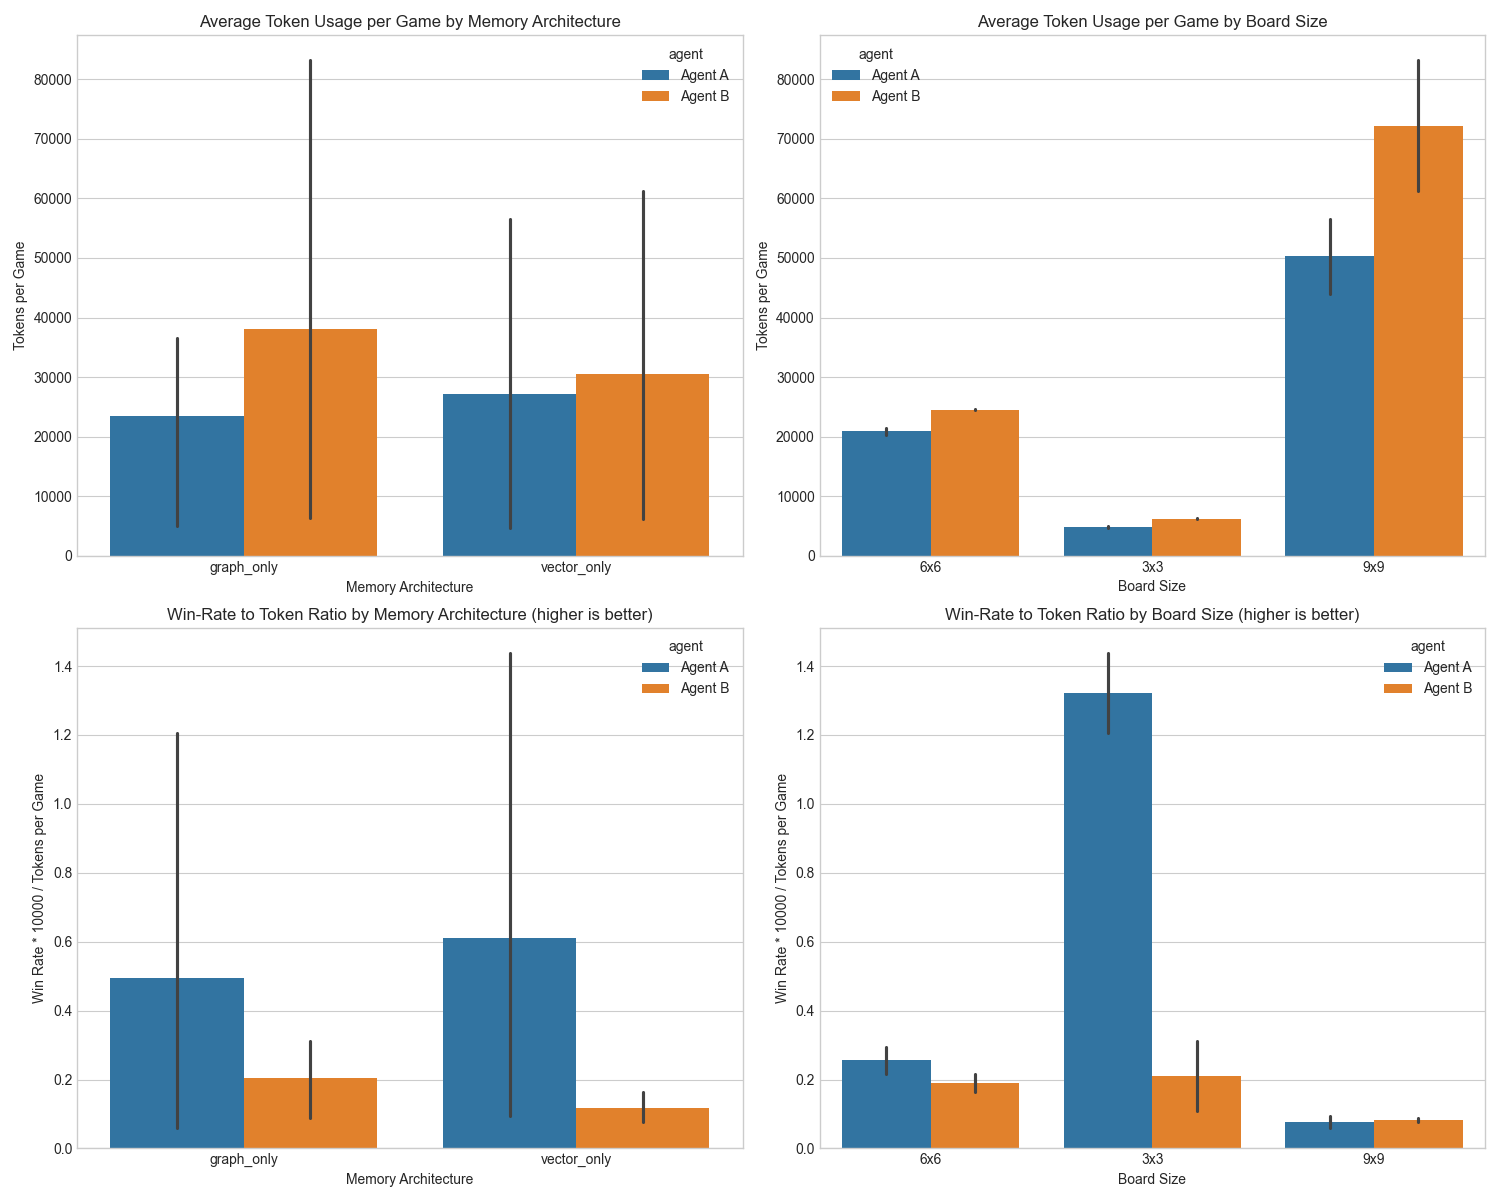
\includegraphics[width=0.9\textwidth]{/Users/diangao/Documents/Workspace/598/CSE-598-Research/experiments/results/analysis/figures/token_efficiency_analysis.png}
    \caption{Token efficiency analysis showing the relationship between token usage and win rates}
    \label{fig:token_efficiency_1}
\end{figure}

\small
\textbf{Finding 1}: Agent A (win-maximizing) consistently makes more memory calls than Agent B (win-token tradeoff) across all experimental conditions.

\textbf{Supporting Data}: Memory call statistics show Agent A making 3-4 times more memory calls than Agent B across all conditions. For example, on 9×9 boards with Vector-only memory, Agent A makes 20 calls versus Agent B's 7 calls.

\textbf{Finding 2}: Agent B uses significantly more tokens per memory call than Agent A, suggesting deeper processing during each memory operation.

\textbf{Supporting Data}: Calculated from token efficiency statistics, Agent B uses 3-5× more tokens per memory call. For example, on 9×9 Graph-only boards, Agent B uses 311,879 tokens per call versus Agent A's 54,916.

\textbf{Hypothesis Assessment}: The first finding supports our hypothesis that Agent A would use memory more frequently. However, the second finding contradicts our expectation that Agent B would have lower token usage overall - instead, it makes fewer but more token-intensive memory calls.

\section{Performance Retention Analysis}

\begin{figure}[t]
    \centering
    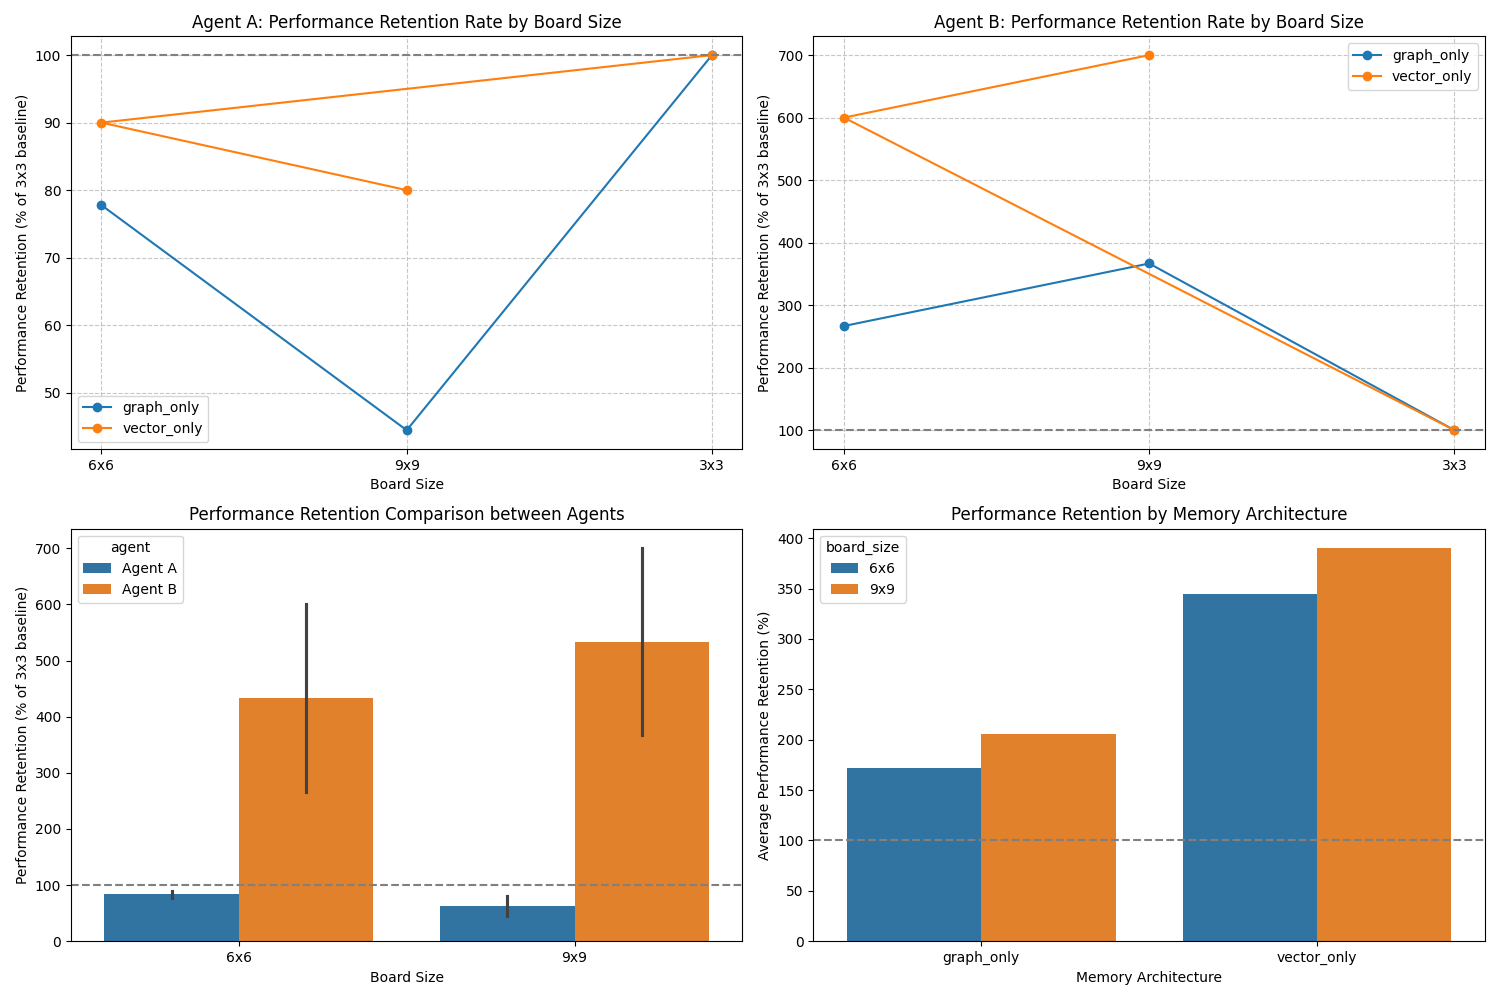
\includegraphics[width=0.9\textwidth]{/Users/diangao/Documents/Workspace/598/CSE-598-Research/experiments/results/analysis/figures/performance_retention_analysis.png}
    \caption{Performance retention across different board sizes and memory architectures}
    \label{fig:performance_retention}
\end{figure}

\small
\textbf{Finding}: Vector memory maintains higher performance levels as board size increases, while Graph memory shows steeper performance decline.

\textbf{Supporting Data}: From 3×3 to 9×9 boards, Agent A's performance retention with Vector memory is 80\% (53.3/66.7) compared to only 44.5\% (26.7/60.0) with Graph memory.

\textbf{Hypothesis Assessment}: This strongly supports our hypothesis that different memory architectures would show varying performance patterns across board sizes, with Vector memory proving more robust for complex state spaces.

\section{Memory-Win Relationship Analysis}

\begin{figure}[t]
    \centering
    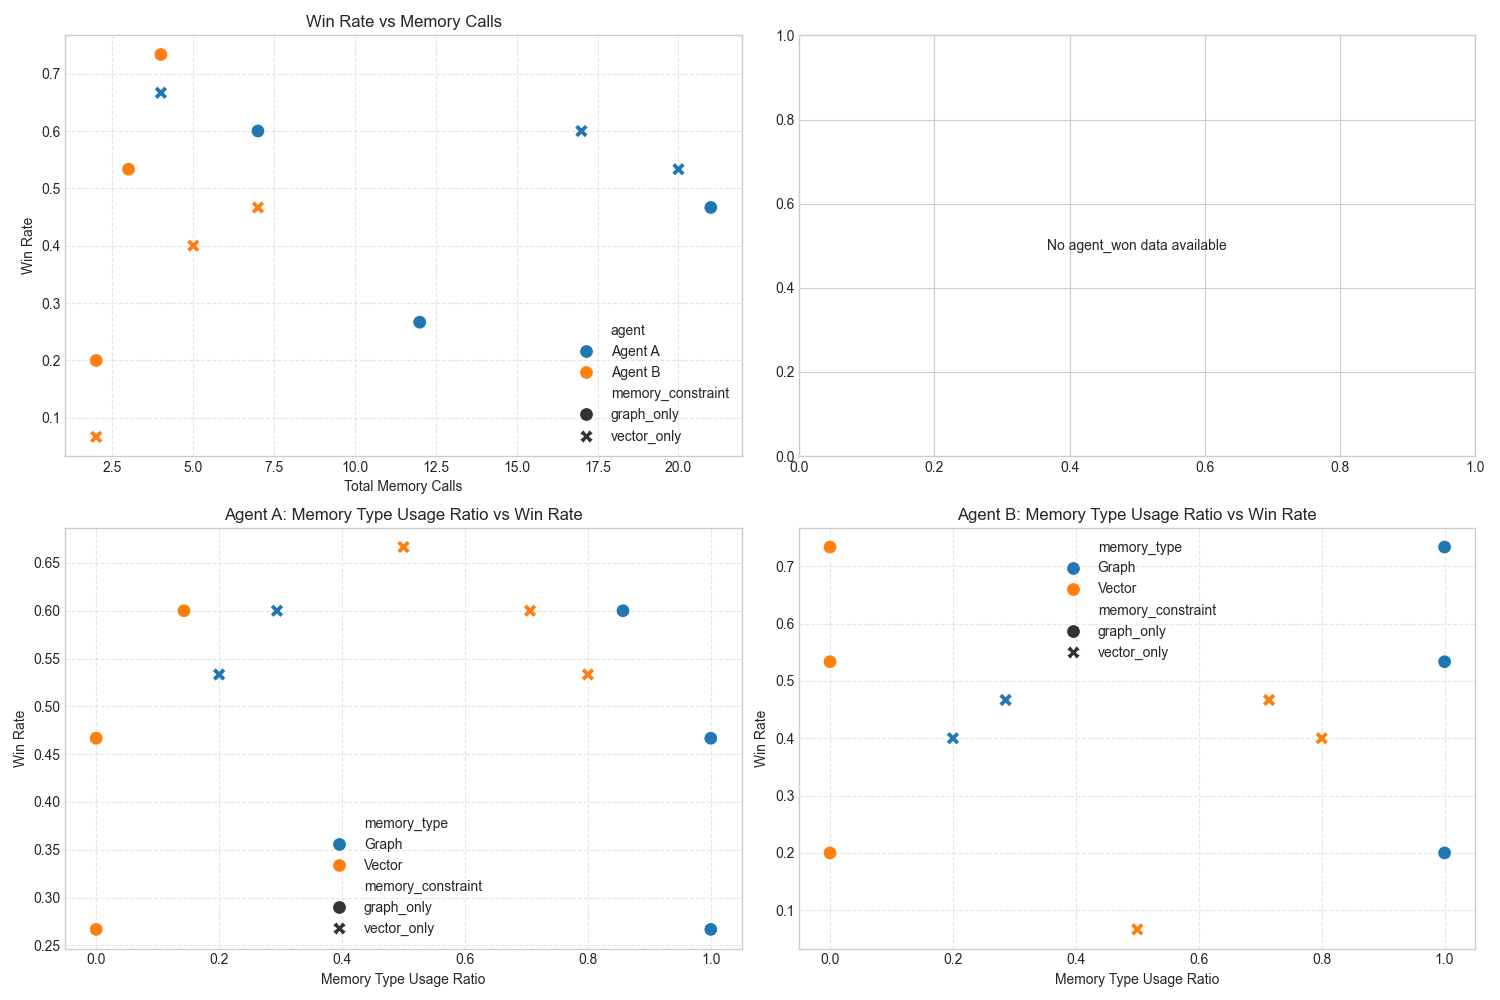
\includegraphics[width=0.9\textwidth]{/Users/diangao/Documents/Workspace/598/CSE-598-Research/experiments/results/analysis/figures/memory_win_relationship.png}
    \caption{Analysis of the relationship between memory usage and win rates}
    \label{fig:memory_win}
\end{figure}

\small
\textbf{Finding}: Memory usage patterns show complex relationships with win rates that vary by memory architecture and board size.

\textbf{Supporting Data}: On 9×9 boards, Agent A's 20 Vector memory calls correlate with a 53.3\% win rate, while its 12 Graph memory calls correlate with only a 26.7\% win rate, suggesting quality and architecture may matter more than quantity.

\textbf{Hypothesis Assessment}: This challenges simplistic views of memory usage and suggests that effective memory utilization depends on both quantity and quality of memory operations, as well as the appropriateness of the memory architecture for the problem complexity.

\section{Conclusions and Implications}
\small
Our visualized analysis provides clear evidence for several key findings:

\subsection{Memory Architecture Effectiveness}
Vector memory consistently outperforms Graph memory across all board sizes, with advantages becoming more pronounced as complexity increases. This contradicts part of our initial hypothesis that predicted Graph memory would excel on smaller boards.

\subsection{Memory Usage Scaling}
Memory requirements generally increase with board size, but Vector memory shows more consistent scaling compared to Graph memory, which peaks at medium complexity before declining. This suggests potential limitations in Graph memory's ability to represent highly complex state spaces effectively.

\subsection{Agent Objective Effects}
Agent optimization objectives significantly impact memory usage strategies. The win-maximizing Agent A uses memory more frequently (higher quantity), while the token-conscious Agent B makes fewer but more token-intensive memory calls (higher quality per call).

\subsection{Adaptive Strategies}
Although our experiments constrained agents to specific memory types, performance differentials strongly suggest that in free-choice scenarios, agents would prefer Vector memory for complex states due to its superior performance on larger boards.

\subsection{Implications for Agent Design}
These findings highlight the importance of matching memory architecture to task complexity and agent objectives. For complex state spaces, Vector memory appears more robust, while for token-constrained applications, a strategy of fewer but more intensive memory operations may be preferable.

\section{Future Work}
\small
Based on our visualized analysis, we recommend several directions for future research:

\begin{enumerate}[leftmargin=*,noitemsep]
    \item Design experiments allowing agents to freely choose between memory types to validate our inferences about adaptive selection
    \item Collect game-phase-specific memory usage data to better understand temporal dynamics of memory utilization
    \item Analyze memory operation content quality rather than just quantity to understand differences in effectiveness
    \item Increase experimental repetitions for greater statistical reliability across different conditions
    \item Extend to other game environments to test the generalizability of our findings about memory architecture effectiveness
\end{enumerate}

\end{document}
